\section{Fase 2: flujo de preprocesamiento}
\label{sec:fase2}

El flujo de preprocesamiento fue \textbf{idéntico para todas las arquitecturas} (salvo cuando
la representación específica de una arquitectura lo exija),
requisito del segundo objetivo específico. Todos los parámetros fueron constantes
del código, sin ajuste por sujeto (tabla~\ref{tab:preproc}).

\begin{longtable}{p{2.9cm}p{3.4cm}p{6.8cm}}
\caption{Parámetros de la cadena de preprocesamiento.}\label{tab:preproc}\\
\toprule
\textbf{Paso} & \textbf{Valor} & \textbf{Justificación} \\
\midrule
\endfirsthead
\toprule
\textbf{Paso} & \textbf{Valor} & \textbf{Justificación} \\
\midrule
\endhead
Filtro pasa banda & \hz{0.5}--\hz{40}, FIR (respuesta finita al impulso) de fase cero (MNE) & Rango frecuencial útil para la detección de tareas de imaginación motora (bandas mu \hz{8}--\hz{13} y beta \hz{13}--\hz{30}) \cite{pfurtscheller1999}. Excluye además de la banda de paso la red eléctrica de \hz{60} y su armónico, por lo que no se aplica un filtro \textit{notch} adicional \\
Remuestreo    & \hz{200} & Captura las frecuencias de imaginación motora (mu y beta) respetando el teorema de Nyquist, con menor costo computacional (menos memoria y cálculo); es además la frecuencia de entrada usada en los trabajos originales de LaBraM y EEGMamba \cite{jiang2024labram,wang2025eegmamba} \\
Montaje      & \texttt{standard\_1005} & Incluye las posiciones del sistema 10-05 presentes en el registro, necesarias para el mapeo espacial de los canales \\
Referencia    & Referencia promedio común (common average reference, CAR) & Requerida por ICLabel para la clasificación de componentes independientes \cite{pion2019iclabel} \\
Artefactos    & ICA (análisis de componentes independientes) + ICLabel & Infomax extendido \cite{lee1999infomax}, 30 componentes, ajustado por \textit{run}; detalle en la sección~\ref{sec:artefactos} \\
Segmentación  & \seg{0.0}--\seg{4.0} tras la señal & Ventana fijada de antemano, de \seg{0} a \seg{4} tras la señal de inicio, que cubre el periodo de la tarea del registro original \cite{lee2019}; no se eligió por exactitud (sección~\ref{sec:ablaciones-f4}) \\
Normalización & \textit{z-score} por canal, ajustado por partición & Los estadísticos se ajustaron solo con el entrenamiento de cada partición, para evitar fuga de datos \\
Aumentación & Desplazamiento temporal de $\pm 5$\,\%, ruido gaussiano al $2$\,\% del canal, máscara de hasta \hz{2} & Se aplicó \textbf{solo al conjunto de entrenamiento} y por minilote, nunca sobre validación ni prueba. Idéntica en las cuatro arquitecturas. La mezcla de segmentos (\textit{mixup}) está implementada pero desactivada \\
\bottomrule
\end{longtable}

La figura~\ref{fig:pipeline} ilustra el flujo: una cadena de preprocesamiento
\textbf{común} a todas las arquitecturas y, al final, la bifurcación en la
representación de entrada específica que consume cada modelo.

\begin{figure}[htbp]
\centering
\begin{tikzpicture}[
  font=\footnotesize,
  paso/.style={draw, rounded corners=2pt, fill=blue!8, minimum width=5.4cm,
               minimum height=0.72cm, align=center},
  rep/.style={draw, rounded corners=2pt, fill=green!12, minimum width=3.0cm,
              minimum height=1.7cm, align=center, font=\scriptsize},
  fl/.style={-{Latex[length=2mm]}, semithick},
  x=1cm, y=1cm
]
%  cadena comun (vertical, centrada en x=0) 
\node[paso] (crudo) at (0, 0)    {Señal cruda: 62 canales, \hz{1000}};
\node[paso] (banda) at (0,-1.0)  {Filtro pasa banda \hz{0.5}--\hz{40} · remuestreo \hz{200}};
\node[paso] (car)   at (0,-2.0)  {Referencia de promedio común (CAR)};
\node[paso] (ica)   at (0,-3.0)  {Eliminación de artefactos: ICA + ICLabel};
\node[paso] (seg)   at (0,-4.0)  {Segmentación \seg{0.0}--\seg{4.0}};
\node[paso, fill=blue!16] (norm) at (0,-5.0) {\textit{z-score} por canal (por partición)};
\node[paso, fill=orange!18] (aug) at (0,-6.0)
  {Aumentación (\textbf{solo entrenamiento})};
\foreach \a/\b in {crudo/banda,banda/car,car/ica,ica/seg,seg/norm,norm/aug}
  \draw[fl] (\a) -- (\b);
\node[anchor=west, font=\scriptsize, align=left] at (3.7,-6.0)
  {desplazamiento $\pm 200$\,ms\\ruido al $2$\,\% del canal\\máscara de hasta \hz{2}};
\node[anchor=west, font=\scriptsize\itshape, align=left] at (3.7,-2.5)
  {Flujo común\\(idéntico para\\todas las\\arquitecturas)};

%  bifurcacion en 4 representaciones 
\node[rep] (eegnet) at (-5.1,-8.0)
  {\textbf{\eegnet{}}\\[2pt]señal cruda\\$C\times T$\\(62 $\times$ 801)};
\node[rep] (conf)   at (-1.7,-8.0)
  {\textbf{Conformer}\\[2pt]señal cruda\\$C\times T$\\(62 $\times$ 801)};
\node[rep] (mamba)  at ( 1.7,-8.0)
  {\textbf{EEGMamba}\\[2pt]parches\\(canales, $n$, 200)};
\node[rep] (labram) at ( 5.1,-8.0)
  {\textbf{LaBraM}\\[2pt]parches (canales, $n$, 200)\\+ índices de canal\\(vocabulario de 128)};
\coordinate (bus) at (0,-6.9);
\draw[fl] (aug) -- (bus);
\foreach \r in {eegnet,conf,mamba,labram}
  \draw[fl] (bus) -| (\r.north);
\end{tikzpicture}
\caption{Flujo de preprocesamiento. La cadena superior es \textbf{común e idéntica}
para todas las arquitecturas. La aumentación se aplicó \textbf{solo al conjunto de
entrenamiento} y por minilote, nunca sobre validación ni prueba; en el último paso se bifurca en la representación de
entrada que requiere cada modelo. \eegnet{} y Conformer consumen la señal cruda
$C\times T$; EEGMamba y LaBraM consumen parches temporales, y LaBraM añade la lista
de índices de canal de su vocabulario de 128 posiciones de electrodo. La cadena corresponde al conjunto principal,
procesado desde la señal cruda; el conjunto externo parte de la versión preprocesada por
sus autores y se armoniza según la sección~\ref{sec:wbcic-preproc}. Las dimensiones de la
bifurcación son las de los protocolos sobre \openbmi{} con sus 62 canales; los modelos del
capítulo~\ref{cap:validacion-externa} reciben los 45 canales comunes a los dos conjuntos.}
\label{fig:pipeline}
\end{figure}

No se aplicó una selección de canales mediante un criterio propio: se utilizaron los
62 canales de \openbmi{} y, en la validación externa, la intersección de 45 canales
comunes a ambos montajes, sin selección por desempeño. La selección de canales espaciales
del segundo objetivo específico quedó implícita en el procesamiento aprendido: la
convolución en profundidad de \eegnet{}, la convolución espacial del Conformer, la
incrustación de identidad de canal de LaBraM y el tratamiento por canal de EEGMamba.
Estos mecanismos no equivalen necesariamente a seleccionar un subconjunto explícito.
Una selección previa guiada por datos sería una decisión ajustada al conjunto de
evaluación y requeriría validación anidada para evitar fuga de información. La prueba
de canales anulados se presenta en el capítulo 5. Los criterios adicionales al desempeño se describieron en la sección~\ref{sec:criterios-adicionales} del capítulo siguiente.


\subsection{Eliminación de artefactos y control del confundidor ocular}
\label{sec:artefactos}

El protocolo de \openbmi{} presenta una particularidad que obliga a un control
explícito: la señal de inicio es \textbf{visual y lateralizada}, y la ventana de
modelado comienza en ella. La sacada ocular hacia el estímulo cae por tanto
dentro de la época, y está correlacionada con la clase por construcción. Un
modelo puede alcanzar exactitud alta decodificando el movimiento ocular en lugar
de la actividad motora imaginada.

Para cuantificarlo se diseñó un control que decodifica la clase usando
\emph{únicamente} una aproximación de electrooculograma construida con los dos canales
frontopolares: una derivación horizontal, $\mathrm{Fp2}-\mathrm{Fp1}$, y una vertical, su
promedio. Sobre ellas se calculó la log-varianza en nueve bandas de \hz{0.5} a \hz{38} y se
clasifica con análisis discriminante lineal (LDA) con contracción, en validación cruzada estratificada de 5 \textit{folds}. Bajo
la hipótesis nula de ausencia de contaminación, ese decodificador debe rendir al
nivel del azar. Se aplicó por sujeto una prueba binomial exacta unilateral ($n = 400$) con
corrección de Holm \cite{holm1979} sobre los 54 sujetos; la prueba supone ensayos
independientes, lo que los ensayos consecutivos de una sesión no cumplen de forma estricta.
La limpieza se realizó con ICA e ICLabel \cite{pion2019iclabel}, implementados en
MNE-Python \cite{gramfort2013mne}: infomax extendido
con 30 componentes, ajustado por \textit{run} sobre la señal continua a \hz{200}, sobre una
copia filtrada desde \hz{1}, en la misma condición
con la que se entrenó ICLabel, y aplicado a la señal de \hz{0.5} a \hz{40}. Se descartan las
componentes clasificadas como oculares con probabilidad $\geq 0.8$, musculares con
$\geq 0.9$ y de ruido de canal con $\geq 0.5$. La tabla~\ref{tab:artefactos} reporta el
efecto de la limpieza.

\begin{table}[htbp]
\centering
\caption{Efecto de la eliminación de artefactos mediante ICA + ICLabel. La exactitud en
canales motores se obtiene con patrones espaciales comunes (CSP) con banco de filtros (FBCSP) y análisis discriminante lineal (LDA) sobre 12 canales.}
\label{tab:artefactos}
\begin{tabular}{lcc}
\toprule
 & \textbf{Sin limpieza} & \textbf{Con limpieza} \\
\midrule
Sujetos con contaminación significativa & 9 / 54 & 4 / 54 \\
Exactitud agregada en canales motores   & $0.774 \pm 0.126$  & $0.750 \pm 0.141$ \\
\bottomrule
\end{tabular}
\end{table}

La atribución espectral separó dos confundidores distintos: siete sujetos con
firma ocular (\hz{0.5}--\hz{8}) y dos con firma muscular ($>\hz{20}$). Se dice que
un sujeto queda \emph{marcado} cuando, tras la limpieza, el control ocular
(decodificador que usa solo la aproximación de electrooculograma, prueba binomial exacta con
corrección de Holm) sigue detectando decodificación significativamente por encima
del azar. Cuatro sujetos quedan marcados: \texttt{sub-06} y \texttt{sub-29}, ya
contaminados antes de la limpieza, persisten; \texttt{sub-32} y \texttt{sub-37}
cruzan el umbral de forma marginal tras el ICA (exactitud del \textit{proxy} ocular
de 0.59 y 0.61 frente al azar de 0.50). Los cuatro se declaran residuales y se
someten al análisis de sensibilidad de la sección~\ref{sec:sensibilidad}.

La tabla~\ref{tab:ablacion} cuantifica el efecto de la limpieza sobre la
exactitud intra-sujeto de \eegnet{}, con la semilla 2026. Se contrasta el grupo contaminado
con un grupo de control de siete sujetos tomados entre los no marcados, sin un criterio de
emparejamiento formal, con el fin de separar el efecto sobre el artefacto del efecto de
perder señal por el propio procedimiento. Los dos grupos parten de niveles distintos
(0.827 frente a 0.613), de modo que esa separación es solo aproximada: el grupo de control,
más cerca del azar, tiene menos margen para bajar.

\begin{table}[htbp]
\centering
\caption{Ablación de la eliminación de artefactos. Exactitud intra-sujeto antes
y después de aplicar ICA + ICLabel, sobre 20 particiones por sujeto.}
\label{tab:ablacion}
\begin{tabular}{llcccc}
\toprule
\textbf{Sujeto} & \textbf{Artefacto} & \textbf{Sin limpieza} & \textbf{Con limpieza}
  & $\boldsymbol{\Delta}$\textbf{ acc} & $\boldsymbol{\Delta}$\textbf{ kappa} \\
\midrule
\multicolumn{6}{l}{\textit{Sujetos contaminados} ($n=9$)} \\
\addlinespace[2pt]
sub-04 & Ocular   & 0.813 & 0.588 & $-0.225$ & $-0.450$ \\
sub-48 & Ocular   & 0.790 & 0.603 & $-0.188$ & $-0.375$ \\
sub-06 & Ocular   & 0.893 & 0.730 & $-0.163$ & $-0.325$ \\
sub-49 & Ocular   & 0.738 & 0.575 & $-0.163$ & $-0.325$ \\
sub-15 & Ocular   & 0.850 & 0.758 & $-0.093$ & $-0.185$ \\
sub-12 & Ocular   & 0.718 & 0.643 & $-0.075$ & $-0.150$ \\
sub-29 & Muscular & 0.923 & 0.850 & $-0.073$ & $-0.145$ \\
sub-35 & Ocular   & 0.973 & 0.903 & $-0.070$ & $-0.140$ \\
sub-07 & Muscular & 0.745 & 0.690 & $-0.055$ & $-0.110$ \\
\addlinespace[3pt]
\multicolumn{2}{l}{\textbf{Media}} & \textbf{0.827} & \textbf{0.704}
  & $\boldsymbol{-0.123}$ & $\boldsymbol{-0.245}$ \\
\midrule
\multicolumn{6}{l}{\textit{Sujetos de control} ($n=7$)} \\
\addlinespace[2pt]
sub-11 &       & 0.598 & 0.533 & $-0.065$ & $-0.130$ \\
sub-13 &       & 0.633 & 0.568 & $-0.065$ & $-0.130$ \\
sub-02 &       & 0.748 & 0.703 & $-0.045$ & $-0.090$ \\
sub-14 &       & 0.588 & 0.555 & $-0.033$ & $-0.065$ \\
sub-18 &       & 0.538 & 0.540 & $+0.003$ & $+0.005$ \\
sub-19 &       & 0.613 & 0.645 & $+0.033$ & $+0.065$ \\
sub-17 &       & 0.575 & 0.630 & $+0.055$ & $+0.110$ \\
\addlinespace[3pt]
\multicolumn{2}{l}{\textbf{Media}} & \textbf{0.613} & \textbf{0.596}
  & $\boldsymbol{-0.017}$ & $\boldsymbol{-0.034}$ \\
\bottomrule
\end{tabular}
\end{table}

La caída es de $-0.123$ en el grupo contaminado (Wilcoxon pareado, $p = 0.004$;
los nueve sujetos bajan) frente a $-0.017$ en el grupo de control, que no alcanza
significancia ($p = 0.375$, calculado con las diferencias redondeadas de la tabla; solo cuatro
de siete bajan). El contraste directo entre las caídas de los dos grupos también es
significativo (Mann-Whitney, $p = 0.002$). La limpieza reduce la exactitud en los sujetos
donde el control detectó artefacto, lo que es compatible con la eliminación de su
contribución ocular o muscular, y apenas modifica la del grupo de control.

Conviene señalar la magnitud de lo que se retiró: en los datos sin limpiar, los
sujetos contaminados promediaban 0.827 frente a 0.613 de los de control. El
artefacto no añadía ruido aleatorio, añadía \emph{desempeño espurio} en sujetos
concretos, que bajo \loso{} son exactamente las particiones de prueba.

\subsection{Verificación de la lectura de los datos contra la literatura}
\label{sec:replica}

Como control de que la carga de los datos, las etiquetas y la partición por sesión son
correctas, se replicó el resultado publicado por los autores con CSP + LDA sobre el mismo
conjunto \cite{lee2019}, empleando su banda, sus canales y su ventana: \hz{8} a \hz{30},
sus 20 canales motores y de \seg{1.0} a \seg{3.5} tras la señal, sin eliminación de
artefactos. La réplica difiere de los autores en tres aspectos: trabaja sobre la señal a
\hz{200} y no a \hz{100}, usa un filtro FIR de fase cero en lugar de su Butterworth de
orden 5, y emplea CSP de 8 componentes con regularización de Ledoit-Wolf y LDA con
contracción. Se evaluó con 10 repeticiones de validación cruzada de 10 \textit{folds} dentro de
cada sesión, que corresponde a la fila CSP-cv de los autores. Se
obtuvieron 0.714 y 0.730 en las sesiones primera y segunda, frente a los 0.701 y 0.722
publicados ($\Delta < 0.015$).

Conviene precisar el alcance de esta réplica. Verifica que el conjunto de datos se lee y se
etiqueta correctamente, pero \textbf{no valida el preprocesamiento de este trabajo}, que
difiere del de los autores en la banda, la frecuencia de muestreo, los canales, la ventana y
la eliminación de artefactos. Para ese preprocesamiento no existe un resultado publicado con
el que contrastarlo directamente; su efecto sobre los datos se documenta en la
sección~\ref{sec:artefactos}.

\subsection{Segundo conjunto de datos: armonización del preprocesamiento}
\label{sec:wbcic-preproc}

La validación externa emplea el subconjunto de dos clases de WBCIC-SHU
\cite{yang2025wbcic}: 51 participantes, 200 segmentos por sesión y 59 canales,
registrado en una institución distinta y con otro amplificador. De sus tres
sesiones se emplea únicamente la primera, por las razones y con las consecuencias
que detalla la sección~\ref{sec:protocolos-extra}.

A diferencia del conjunto principal, que se procesa en este trabajo desde la señal cruda,
WBCIC-SHU se toma de la \textbf{versión preprocesada que distribuyen sus autores}: ya
filtrada entre \hz{0.5} y \hz{40}, con un filtro de rechazo de banda entre \hz{49} y \hz{51}
para la red eléctrica de \hz{50}, referenciada a Pz, a \hz{250} y con la media de cada
segmento sustraída. La armonización se aplicó sobre esos datos.

El objetivo de esta armonización no es preprocesar bien ese conjunto por separado,
sino que ambos lleguen a la red habiendo recibido el mismo tratamiento. De lo
contrario, la diferencia de desempeño mediría el preprocesamiento en lugar del
cambio de dominio. La tabla~\ref{tab:armonizacion} resume paso a paso qué se pudo
igualar y qué no.

\needspace{8\baselineskip}

{\small
\begin{longtable}{@{}p{3.0cm}p{3.2cm}p{7.4cm}@{}}
\caption{Armonización del preprocesamiento entre los dos conjuntos de datos. Las
seis últimas filas son las diferencias que no se pudieron eliminar.}
\label{tab:armonizacion}\\
\toprule
\textbf{Paso} & \textbf{Estado} & \textbf{Tratamiento} \\
\midrule
\endfirsthead
\toprule
\textbf{Paso} & \textbf{Estado} & \textbf{Tratamiento} \\
\midrule
\endhead
Segmentación & Idéntica & \seg{0.0}--\seg{4.0} tras la señal de inicio \\
Remuestreo & Igualado & De \hz{250} a \hz{200} \\
Eliminación de artefactos & Mismos parámetros & ICA por infomax extendido, 30 componentes, misma semilla y los mismos umbrales de ICLabel \\
Canales & Intersección & 45 canales comunes a los dos montajes, en idéntico orden. Se descartan 17 del conjunto principal, entre ellos su serie de alta densidad, y 14 del externo \\
\midrule
Referencia & \textbf{Mismo procedimiento, distinto conjunto de electrodos} & El conjunto externo se distribuyó referenciado a Pz, que queda anulado. Reinsertando ese canal como fila de ceros y al aplicar el promedio común sobre los 59 se recuperó exactamente su CAR, porque $(x_i - x_{Pz}) - \overline{(x_j - x_{Pz})} = x_i - \overline{x_j}$. El promedio se calculó, sin embargo, sobre los 59 electrodos del externo y los 62 del principal, de modo que las dos referencias no son la misma combinación de electrodos \\
Filtro pasa banda & \textbf{Misma banda, distinto filtro} & Ambos estuvieron en \hz{0.5}--\hz{40}, pero el conjunto externo llegó filtrado por sus autores y el principal se filtró en este trabajo, de modo que coincide la banda y no necesariamente la respuesta del filtro. El externo incluye además un rechazo de banda entre \hz{49} y \hz{51}, que cae fuera de la banda útil \\
Corrección de línea base & \textbf{No igualable} & El conjunto externo se distribuye con la media de cada segmento ya sustraída. Igualarlo exigiría reconstruir el conjunto principal e invalidaría los resultados ya obtenidos \\
Ajuste del ICA & \textbf{No igualable} & En el conjunto principal se ajusta por ejecución sobre la señal continua; en el externo, por sujeto sobre segmentos, porque las marcas de evento no son legibles sin el lector propietario del fabricante \\
Rechazo por amplitud & \textbf{Asimétrico} & Ver la discusión siguiente \\
Sesiones por sujeto & \textbf{No igualable} & \openbmi{} aporta sus dos sesiones y WBCIC-SHU solo la primera de sus tres, de modo que un modelo nativo del segundo entrena con 144 segmentos por persona frente a 360. Igualarlo exigiría reprocesar las dos sesiones restantes; se declara y se tiene en cuenta al interpretar (sección~\ref{sec:protocolos-extra}) \\
\bottomrule
\end{longtable}
}

\textbf{Sobre el rechazo por amplitud.} El conjunto principal no aplica ningún
rechazo de segmentos por umbral de amplitud, en coherencia con los trabajos publicados sobre él.
En el conjunto externo se descartan los segmentos cuyo pico supere los
$5\,000$~$\mu$V. La asimetría se declara aquí porque afecta a un solo
conjunto, pero conviene precisar su alcance real: el criterio elimina
\textbf{un segmento de 10\,199}, el 0.01\,\% de los datos.

La razón para no conservarlo es que ese segmento no contiene señal
electroencefalográfica sino saturación del amplificador, con un pico de
$78\,477$~$\mu$V en el canal O1 frente a un máximo mediano de
$50$~$\mu$V en el resto de segmentos de ese mismo participante.
Conservarlo tampoco es neutro: la desviación típica se calcula como una suma de
cuadrados, de modo que ese único valor aporta el 99.5\,\% de la suma del canal y
los 10\,198 segmentos restantes el 0.5\,\%. La desviación típica de O1 pasa de
$19.5$~$\mu$V a $274.5$~$\mu$V, y al normalizar, la señal
útil de ese canal queda comprimida al 7\,\% de su escala. Por la referencia
promedio el efecto se propaga: 43 de los 45 canales ven su desviación típica
inflada más de un 5\,\%. Descartar un segmento entre diez mil es una intervención
menor comparada con normalizar todo el conjunto con un estadístico dominado por un
fallo de instrumentación.

\subsection{Variantes de preprocesamiento evaluadas}
\label{sec:variantes-preproc}

Además del preprocesamiento común se evaluaron variantes: más semillas, aumentación de datos, alineamiento de covarianzas, subbandas y ventanas, y un
escenario de calibración con pocos ensayos. Esta subsección describe las variantes de
preprocesamiento; las semillas y la aumentación se describen en la
sección~\ref{sec:fase3-variantes}, y la calibración en la sección~\ref{sec:metodo-fewshot}.
Cada variante conserva los datos, el preprocesamiento común, las particiones y la
configuración de entrenamiento de su arquitectura, y se compara con la ejecución base
\emph{de la misma semilla} en contraste pareado por sujeto.

\subsubsection{Subbandas y ventanas}
\label{sec:variantes-banda}

El preprocesamiento común filtra una sola banda de \hz{0.5} a \hz{40}
(tabla~\ref{tab:preproc}). Para evaluar la dependencia de los resultados de la banda y de
la ventana se derivan variantes del mismo conjunto de segmentos, en el protocolo
intra-sujeto.

\begin{itemize}
  \item \textbf{Subbandas.} Mu (\hz{8} a \hz{13}), beta (\hz{13} a \hz{30}) y mu más beta
  (\hz{8} a \hz{30}). Se aplica un filtro Butterworth de orden $4$ de forma bidireccional (fase cero), con relleno par de un segundo, a todo el segmento guardado en
  la memoria intermedia, que abarca de \seg{-0.5} a \seg{4.5}, y después se recorta a la
  ventana de \seg{0} a \seg{4}. De ese modo los transitorios de borde quedan fuera de la
  ventana de modelado. Es un filtro en cascada sobre datos ya filtrados de \hz{0.5} a
  \hz{40} y limpios de ICA, no un preprocesamiento rehecho desde el registro original. Los
  estadísticos de normalización se recalculan sobre la señal filtrada.
  \item \textbf{Ventanas.} De \seg{0} a \seg{2} ($401$ muestras) y de \seg{0} a \seg{3}
  ($601$ muestras), recortadas del mismo segmento guardado, con la banda base. La
  aumentación por desplazamiento temporal conserva su fracción del $5$\,\% de la ventana,
  de modo que el desplazamiento máximo es de $\pm 20$ muestras ($100$\,ms) en la ventana de
  \seg{2} y de $\pm 30$ ($150$\,ms) en la de \seg{3}, frente a $\pm 40$. Con parches de
  \seg{1}, la ventana de \seg{2} da a LaBraM dos parches en lugar de cuatro.
\end{itemize}

Cada variante usó la semilla $2026$. La banda y la ventana se evaluaron solo en intra-sujeto.
La banda conjunta de \hz{8} a \hz{30} se evaluó en \eegnet{} y el Conformer; se omitió
en LaBraM y EEGMamba por costo de cómputo, al igual que las demás subbandas
(sección~\ref{sec:ablaciones-recortadas}).

El filtro de banda ancha de \hz{0.5} a \hz{40} es FIR (respuesta finita al impulso) de fase cero de MNE,
diseñado con \texttt{firwin}. Las subbandas emplean un Butterworth IIR (respuesta infinita al impulso) de orden 4,
aplicado en ida y vuelta mediante \texttt{sosfiltfilt}, también de fase cero y de
orden efectivo 8. En la comparación de respuestas de magnitud calculada con
\texttt{scripts/informe\_filtros\_fir\_iir.py}, la atenuación FIR en los bordes
inferior y superior fue, respectivamente, 0.023 y 0.044 dB para mu, 0.028 y
0.029 dB para beta, y 0.032 y 0.037 dB para mu más beta. La IIR presentó
6.021 dB en cada corte nominal por la doble pasada; MNE sitúa la transición FIR
fuera de los bordes nominales (figura~\ref{fig:filtros-fir-iir}).

\begin{figure}[htbp]
\centering
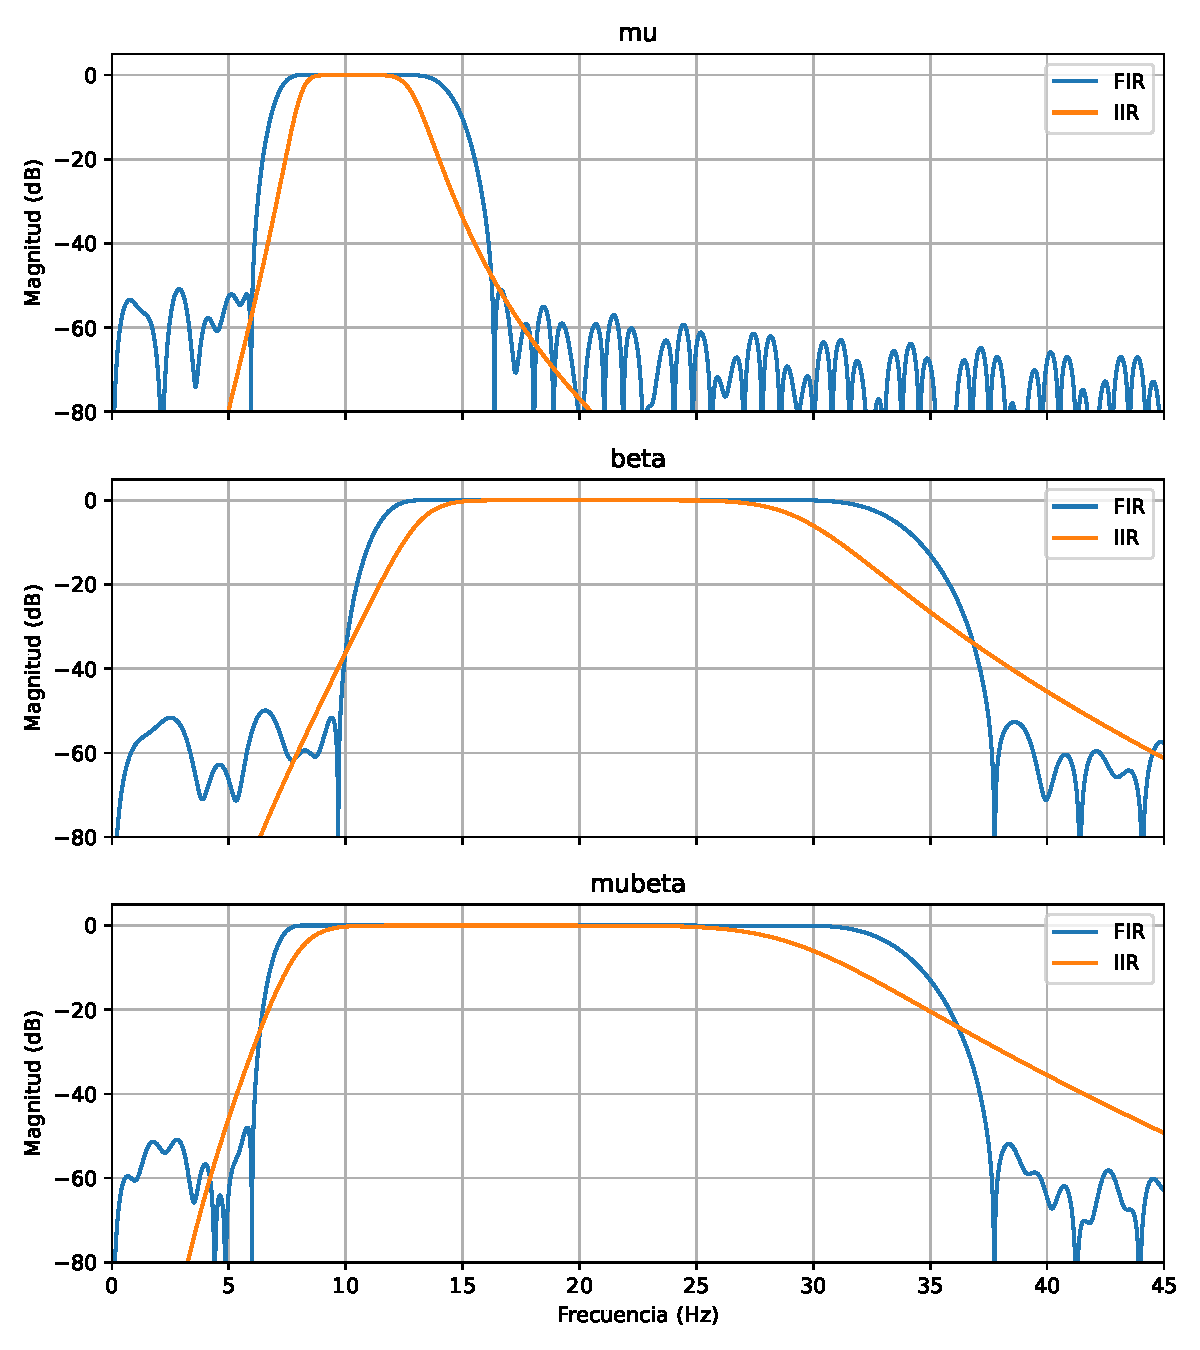
\includegraphics[width=0.95\textwidth]{figuras/filtros_fir_iir.pdf}
\caption{Comparación de las respuestas de magnitud de los filtros FIR e IIR de fase cero para las subbandas mu, beta y mu más beta.}
\label{fig:filtros-fir-iir}
\end{figure}

Para aislar el efecto del tipo de filtro se repitieron las tres subbandas en \eegnet{}
intra-sujeto, con la semilla 2026, filtradas mediante FIR (respuesta finita al impulso) de fase cero.
% PENDIENTE-E1: resultado

\subsubsection{Alineamiento euclidiano}
\label{sec:variantes-ea}

Se evaluó el alineamiento euclidiano de covarianzas \cite{he2020ea} como corrección de las
diferencias entre sujetos y entre conjuntos de datos que la normalización por canal no
alcanza. Para cada sujeto se calculó la covarianza espacial media de sus segmentos, según la ecuación~\eqref{eq:covarianza-media}:
\begin{equation}
  R = \frac{1}{n}\sum_{i=1}^{n}\frac{X_i X_i^{\top}}{T},
  \label{eq:covarianza-media}
\end{equation}
con $X_i \in \mathbb{R}^{C \times T}$ el segmento $i$ (ventana de \seg{0} a \seg{4}, las
dos sesiones) y $n$ el número de segmentos del sujeto, y cada segmento se transforma como
$X_i \leftarrow R^{-1/2} X_i$. La transformación se aplicó a todos los sujetos, de
entrenamiento y de prueba, antes de la normalización por canal con los estadísticos del
entrenamiento, que se mantiene. No emplea etiquetas.

Dos decisiones de implementación. Primera, la referencia promedio y la eliminación de
componentes por ICA hacen que $R$ no sea de rango completo, de modo que la raíz inversa se
calcula con la pseudoinversa: se diagonaliza $R$, se conservan los autovalores mayores que
$10^{-6}$ veces el mayor y se anulan los demás. Segunda, el alineamiento depende de los
canales que entran en la covarianza, así que se calculó una vez por vista de canales: con
los $62$ canales para \loso{} y con los $45$ canales comunes para la transferencia, el
modelo nativo y los sujetos apartados, en ambos conjuntos de datos.

No se emplea el alineamiento riemanniano \cite{zanini2018}, que exige matrices de
covarianza definidas positivas; las de este conjunto no lo son por las razones del párrafo
anterior.

\textbf{El alineamiento es transductivo.} El sujeto de prueba se alinea con la covarianza de
sus propios segmentos sin etiqueta, todos y no solo unos pocos, igual que la política de
normalización por sujeto de la sección~\ref{sec:protocolos-extra}. Los resultados con
alineamiento no son por tanto \textit{zero-shot} en sentido estricto: suponen disponer de los
registros del sujeto antes de clasificar. El alineamiento se evaluó con la semilla $2026$ en
\loso{}, la transferencia, el modelo nativo y los sujetos apartados, con recorte de
gradiente.

